
%-------------------------------------------------------------------------------
%							THIRD SECTION
%-------------------------------------------------------------------------------

\section{Results}



% %% Template
% \begin{columns}[T]
%     \begin{column}{.48\textwidth}
%     \color{purple}\rule{\linewidth}{4pt}
%     Classic FEM \color{black}

%     \end{column}%
%     \hfill%
%     \begin{column}{.48\textwidth}
%     \color{orange}\rule{\linewidth}{4pt}
%     \phifem \color{black}

%     \end{column}%
% \end{columns}


\subsection{The Poisson problem}

\begin{frame}[t]
    \frametitle{Theoretical framework for the Poisson problem} The Poisson problem:
    \Large 
    \begin{align} 
        \begin{cases}
            -\Delta u = f  &\quad \text{in } \Omega \\
            u = 0  &\quad \text{on } \partial\Omega 
        \end{cases}
        \label{eq:poisson}
    \end{align}
    % \vspace*{0.1cm}
    \normalsize
    \pause
\begin{columns}[T] % align columns
    \begin{column}{.46\textwidth}
        \color{purple}\rule{\linewidth}{4pt}
        Classic FEM
        \color{black} \\ \footnotesize \vspace*{1pt}
        Find $u_h \in V_h^{(k)}$ such that
        \begin{align*}
            a_h(u_h,v_h)=l_h(v_h), \,\, \forall \, v_h \in V_h^{(k)},
        \end{align*}
        where
        \begin{align*}
            \notag
            a_h(u,v) & = \int_{\Omega_h} \nabla u \cdot \nabla v \\
            l_h(v) &= \int_{\Omega_h} fv \,.
            \label{eq:PoissonClassic}
        \end{align*}
        \hrule
    \end{column}%

    \hfill%
    
    \normalsize

    \pause
    \begin{column}{.50\textwidth}
        \color{orange}\rule{\linewidth}{4pt}
        \phifem 
        \color{black} \footnotesize (\cite{Reference3}) \\ \vspace*{1pt}
        First, write $u_h = \phi_h w_h$. Then find $w_h\in V_h^{(k)}$ such that
        \begin{equation*}
          a_h(w_h,v_h)=l_h(v_h)\mbox{ for all }v_h\in V_h^{(k)},
        \end{equation*}
        where
        \begin{equation*}
           a_h(w,v)=\displaystyle \int_{\Omega_h} \nabla (\phi_h w) \cdot \nabla (\phi_h v) -
           \textcolor{brown}{\int_{\partial \Omega_h} \frac{\partial}{\partial n} (\phi_h w) \phi_h
           v} + \textcolor{blue}{G_h (w, v)} 
        \end{equation*}	
           \[\displaystyle   l_h(v) = \int_{\Omega_h} f \phi_h v + \textcolor{red}{G_h^{rhs} (v)}. \]
    \end{column}%
\end{columns}
\pause
\footnotesize
\begin{align*} 
    \textcolor{blue}{G_h(w, v)} &: = \displaystyle\sigma h\sum_{E\in  \mathcal{F}_h^{\Gamma}} 
\int_E \left[ \frac{\partial}{\partial n}
   (\phi_h w) \right] \left[ \frac{\partial}{\partial n} ( \phi_hv)\right] + \sigma h^2 \sum_{T \in \Th^{\Gamma}} \int_T \Delta(\phi_h w) \Delta(\phi_h v)  
    \,, \\
    \textcolor{red}{G_h^{rhs} (v)} &: =\displaystyle- \sigma h^2\sum_{T \in\Th^{\Gamma}} \int_T f \Delta (\phi_h v)   
   \,.
\end{align*}

\end{frame}


\begin{frame}
    \frametitle{Numerical solution for the Poisson problem}

    \begin{columns}[T] % align columns
        \begin{column}{.48\textwidth}
        \color{purple}\rule{\linewidth}{4pt}
        Classic FEM \color{black}
        \begin{align*}
            \begin{cases}
            \Omega = \left\{ (x,y)\in\mathbb{R}^2: \left( x-\frac{1}{2} \right)^2 + \left( y-\frac{1}{2} \right)^2 < \frac{1}{8}  \right\} \\
            u(x,y)= -\left( \frac{1}{8} - \left( x-\frac{1}{2} \right)^2 - \left( y-\frac{1}{2} \right)^2 \right) \exp(x) \sin(2\pi y)\\
            f(x,y) = -\frac{\partial^2 u}{\partial x^2}(x,y) -\frac{\partial^2 u}{\partial y^2}(x,y)
            \end{cases}
        \end{align*}
        
        \end{column}%
        \hfill%
        \begin{column}{.48\textwidth}
        \color{orange}\rule{\linewidth}{4pt}
        \phifem \color{black}
        \begin{align*}
            \begin{cases}
            \mathcal{O} = [0,1]\times[0,1] \\
            \phi(x,y) = -\frac{1}{8} + \left( x-\frac{1}{2} \right)^2 + \left( y-\frac{1}{2} \right)^2 \\
            u(x,y)=\phi(x,y) \times \exp(x) \times \sin(2\pi y) \\
            f(x,y) = -\frac{\partial^2 u}{\partial x^2}(x,y) -\frac{\partial^2 u}{\partial y^2}(x,y) \\
            \sigma = 20
            \end{cases}
        \end{align*}
        
        \end{column}%
    \end{columns}

    \pause

    \begin{columns}
        \begin{column}{0.48\textwidth}
            \centering
            \begin{figure}            
            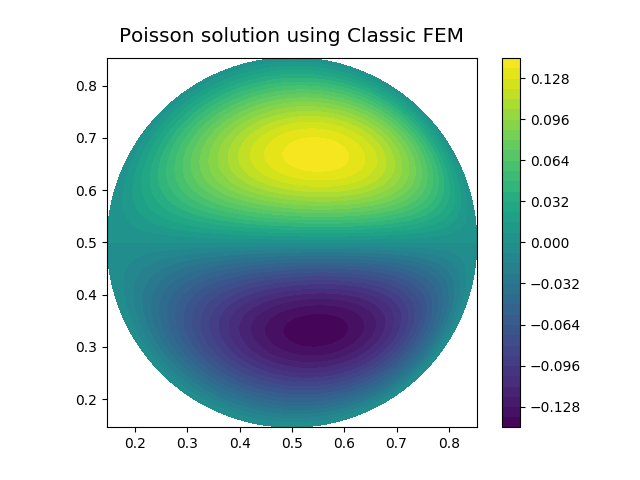
\includegraphics[width=0.95\textwidth]{ClassicSol2.png}
            \caption{Classic FEM ($39642$ cells)}
            \end{figure}
        \end{column}
        \begin{column}{0.48\textwidth}
            \centering
            \begin{figure}            
            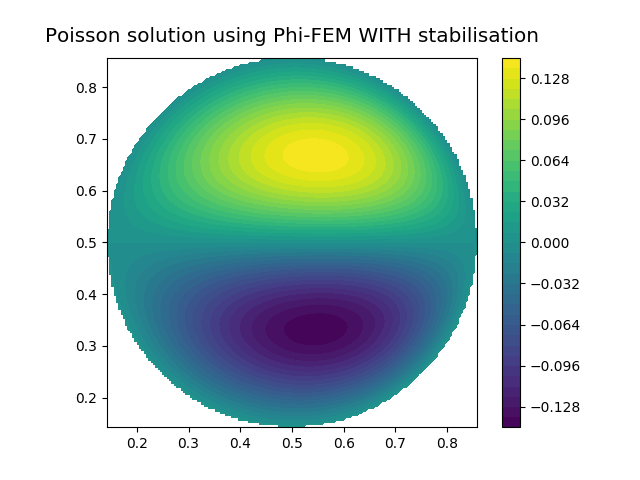
\includegraphics[width=0.95\textwidth]{StabSol.png}
            \caption{\phifem ($39936$ cells)}
            \end{figure}
        \end{column}
    \end{columns}

    \note{Remarque sur la non-smoothness de la solution sur les bords. C'est parcequ'un disque c'est facilement maillable!}

\end{frame}

\begin{frame}
    \frametitle{Convergence study for the Poisson Problem}

\begin{columns}
    \begin{column}{0.48\textwidth}
        \centering
        \begin{figure}            
        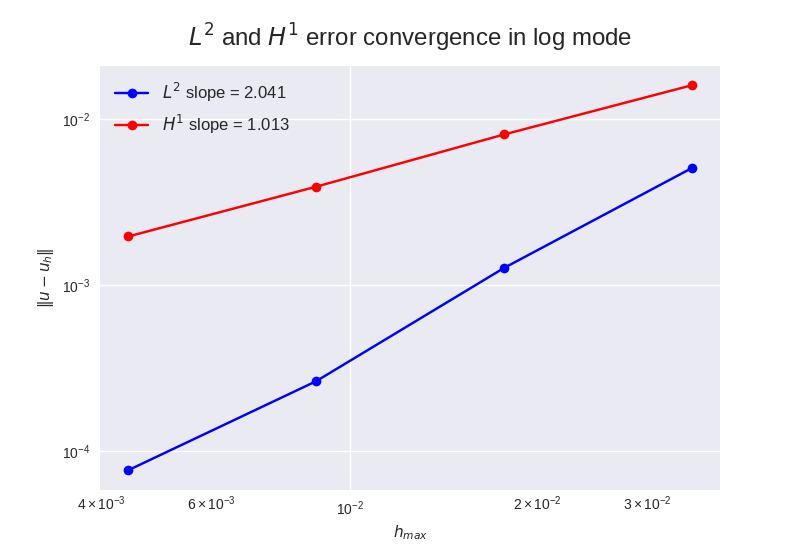
\includegraphics[width=0.95\textwidth]{ClassicCvgStudy2.png}
        \caption{Classic FEM}
        \end{figure}
    \end{column}
    \begin{column}{0.48\textwidth}
        \centering
        \begin{figure}            
        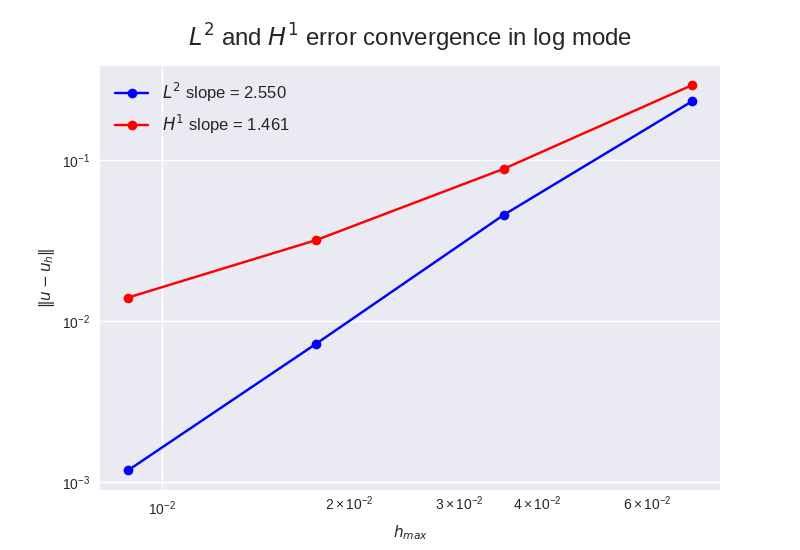
\includegraphics[width=0.95\textwidth]{StabCvgStudy.png}
        \caption{\phifem}
        \end{figure}
    \end{column}
\end{columns}

\begin{table}[h!]
    \centering
    \begin{tabular}{c| l| c| c}
        \toprule
        \tabhead{Problem} & \tabhead{Technique} & \tabhead{$L^2$ slope} & \tabhead{$H^1$ slope} \\
        \midrule
        \multirow{2}{4em}{Poisson} & Classic FEM & 2.041 & 1.013 \\
         & \phifem & 2.550 & 1.461 \\
        \bottomrule
    \end{tabular}
    \caption{Convergence rates.}
  \end{table}

\end{frame}






\subsection{The elasticity equation}

\begin{frame}[t]
    \frametitle{Theoretical framework for the elasticity equation} The elasticity equation: \large
    \begin{align}
        \begin{cases}
        \nabla \cdot \sigma(u) + f = 0 &\quad \text{in } \Omega\\   
        \sigma(u) = \lambda(\nabla \cdot u) \mathcal{I} + \mu (\nabla u + \nabla u^T)  &\quad \text{in } \Omega\\
        u = g &\quad \text{on } \partial\Omega
        \end{cases}
        \label{eq:elasticity}
    \end{align}
    % \vspace*{0.1cm}
    \normalsize

    \pause

    \note{Rappler qu'il s'agit d'une formulation variationnelle dans l'espace H1, et non l'approximation éléments finis. Ce qui fait qu'on peut enlever le subscript h. }

\begin{columns}[T] % align columns
    \begin{column}{.44\textwidth}
        \color{purple}\rule{\linewidth}{4pt}
        Classic FEM
        \color{black} \\ \footnotesize
        First $V=\left[H_0^1(\Omega)\right]^d$, and $\gamma G = g$. Then find $u \in G + V $ such that
        \begin{align*}
         a(u,v)=l(v), \quad \forall v \in V
        \end{align*}
        where $a$ and $l$ are defined as 
        $$
        a(u,v) = \int_{\Omega} \sigma (u) : \varepsilon (v)
        $$
        and
        $$
        l(v) = \int_{\Omega} f\cdot v
        $$
    \hrule
    \end{column}%

    \hfill%
    \pause
    
    \normalsize
    \begin{column}{.52\textwidth}
        \color{orange}\rule{\linewidth}{4pt}
        \phifem 
        \color{black} \\ \footnotesize
        First, $u_h = \phi w + g$. Then find $w \in V$ such that:
        \begin{align*}
            a(w,v)=l(v), \quad \forall v \in V
        \end{align*}
        where $a$ and $l$ are defined as 
        $$
        a(w,v) = \int_{\Omega} \sigma(\phi w) : \varepsilon(\phi v) - \textcolor{brown}{\int_{\partial\Omega} (\sigma(\phi w) \cdot n) \cdot (\phi v)} + \textcolor{blue}{G(w,v)}
        $$
        and
        $$
        l(v) = \int_{\Omega} f \cdot (\phi v) + \textcolor{teal}{\int_{\partial\Omega} (\sigma(g) \cdot n) \cdot (\phi v)} - \textcolor{magenta}{\int_{\Omega} \sigma(g) : \varepsilon(\phi v)} + \textcolor{red}{G_{rhs}(v)}
        $$        
    \end{column}%
\end{columns}
\pause
\footnotesize
$$
\textcolor{blue}{G(w,v)} = \sigma_{pen} h^2 \sum_{E \in \mathcal{T}_h^{\Gamma}} \int_{E} \left(\nabla \cdot \sigma(\phi w)\right) \cdot \left( \nabla \cdot \sigma(\phi v)\right) + \sigma_{pen} h \sum_{F \in \mathcal{F}_h^{\Gamma}} \int_{F} \left[\sigma(\phi w) \cdot n \right] \cdot \left[ \sigma(\phi v) \cdot n \right] 
$$ 

$$
\textcolor{red}{G_{rhs}(v)} = - \sigma_{pen} h^2 \sum_{E \in \mathcal{T}_h^{\Gamma}} \int_{E} \left( f + \nabla \cdot \sigma(g) \right) \cdot \left( \nabla \cdot \sigma(\phi v)\right) - \sigma_{pen} h \sum_{F \in \mathcal{F}_h^{\Gamma}} \int_{F} \left[\sigma(g) \cdot n \right] \cdot \left[ \sigma(\phi v) \cdot n \right]
$$


\end{frame}

\small

\begin{frame}
    \frametitle{Numerical solution for the elasticity equation}

    \begin{columns}[T] % align columns
        \begin{column}{.48\textwidth}
        \color{purple}\rule{\linewidth}{4pt}
        Classic FEM \color{black}
        \begin{align*}
            \begin{cases}
            \Omega = \left\{ (x,y)\in\mathbb{R}^2: \left( x-\frac{1}{2} \right)^2 + \left( y-\frac{1}{2} \right)^2 < \frac{1}{8}  \right\} \\
            u(x,y)= \begin{pmatrix}
                2x + \sin(x)\exp(y) \\ \frac{x}{2} + \cos(x) - 1
            \end{pmatrix}  \\
            f(x,y) = -\nabla \cdot \sigma(u(x,y)) \\
            g(x,y) = u(x,y)
            \end{cases}
        \end{align*}
        
        \note{Signaler que g n'est pas egale à u sur les bords, ceci afin d'introduire une perturbation qui sera résolue par les termes de penalisation.}

        \end{column}%
        \hfill%
        \begin{column}{.48\textwidth}
        \color{orange}\rule{\linewidth}{4pt}
        \phifem \color{black}
        \begin{align*}
            \begin{cases}
            \mathcal{O} = [0,1]\times[0,1] \\
            \phi(x,y) = -\frac{1}{8} + \left( x-\frac{1}{2} \right)^2 + \left( y-\frac{1}{2} \right)^2 \\
            u(x,y)= \begin{pmatrix}
                2x + \sin(x)\exp(y) \\ \frac{x}{2} + \cos(x) - 1
            \end{pmatrix}  \\
            f(x,y) = -\nabla \cdot \sigma(u(x,y)) \\
            g(x,y) = u(x,y) + \textcolor{blue}{\phi(x,y) \begin{pmatrix}
               \sin(x) \\ \exp(y)
            \end{pmatrix}} \\
            \sigma_{pen} = 20
            \end{cases}
        \end{align*}
        

        \end{column}%
    \end{columns}

    \pause

    \begin{columns}
        \begin{column}{0.4\textwidth}
            \centering
            \begin{figure}            
            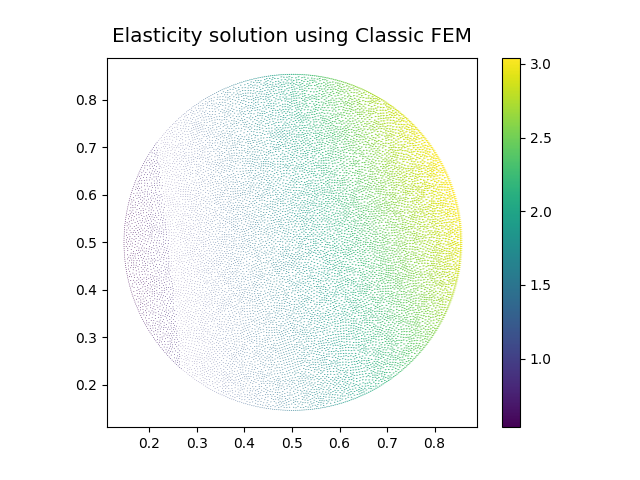
\includegraphics[width=0.95\textwidth]{ClassicElasSol.png}
            \caption{Classic FEM}
            \end{figure}
        \end{column}
        \begin{column}{0.4\textwidth}
            \centering
            \begin{figure}            
            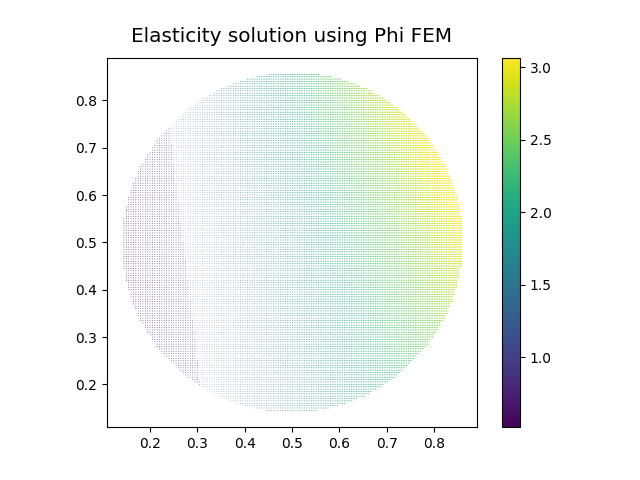
\includegraphics[width=0.95\textwidth]{StabElasSol.png}
            \caption{\phifem}
            \end{figure}
        \end{column}
    \end{columns}

\end{frame}

\begin{frame}
    \frametitle{Numerical solution for the elasticity equation (cont.)}

    \begin{figure}[H]
        % \centering
        \begin{subfigure}{0.2\textwidth}
            % \centering
            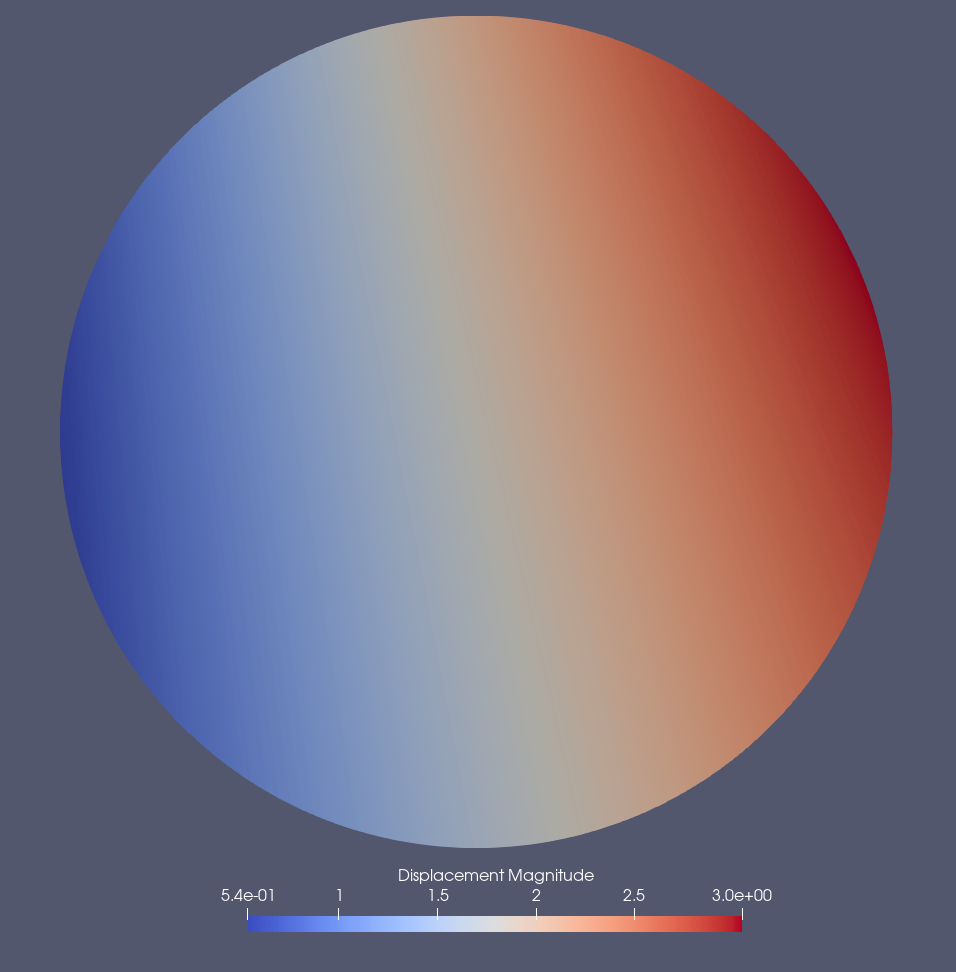
\includegraphics[width=\textwidth]{ClassicElasPara1.png}
          \caption{Classic FEM}
        \end{subfigure}
        \begin{subfigure}{0.21\textwidth}
            % \centering
            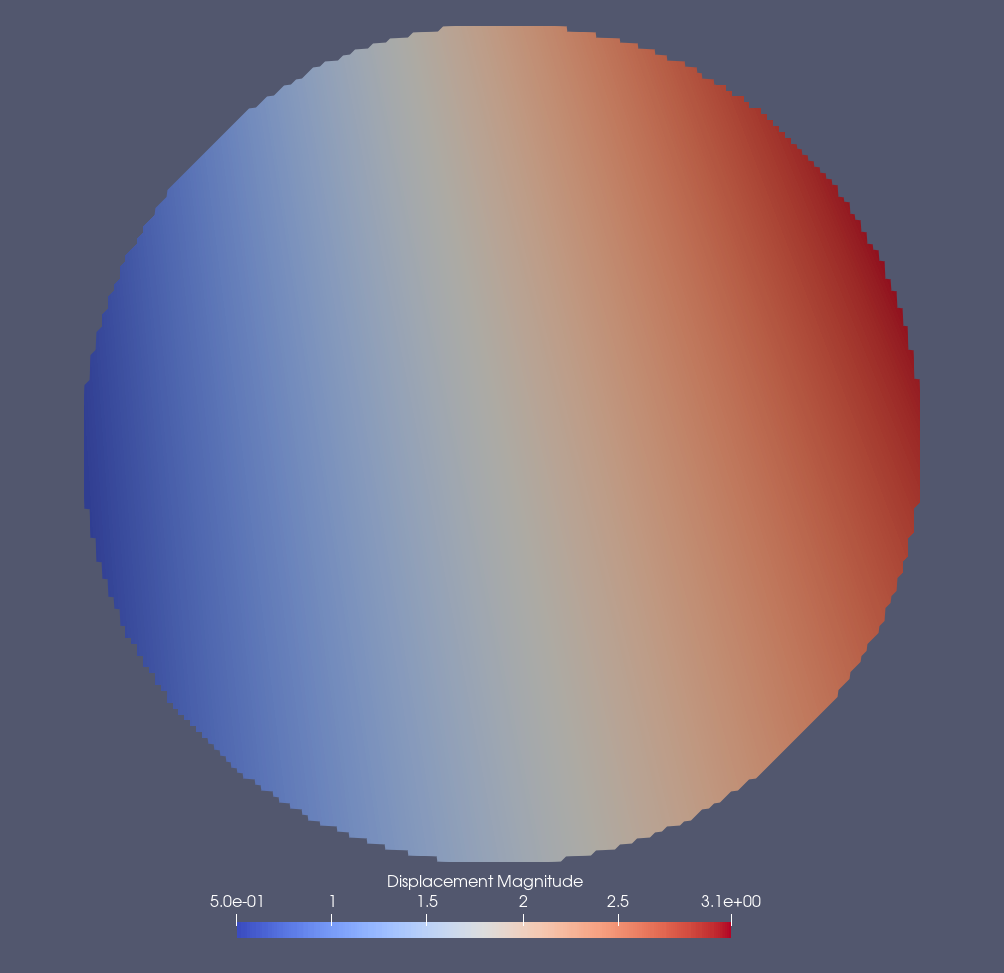
\includegraphics[width=\textwidth]{StabElasPara1.png}
          \caption{\phifem}
        \end{subfigure}
        \caption{Solution (deformation) magnitude in Paraview.}
    \end{figure}
    
    \zerodisplayskips
    \begin{figure}[H]
        % \centering
        \begin{subfigure}{0.2\textwidth}
            % \centering
            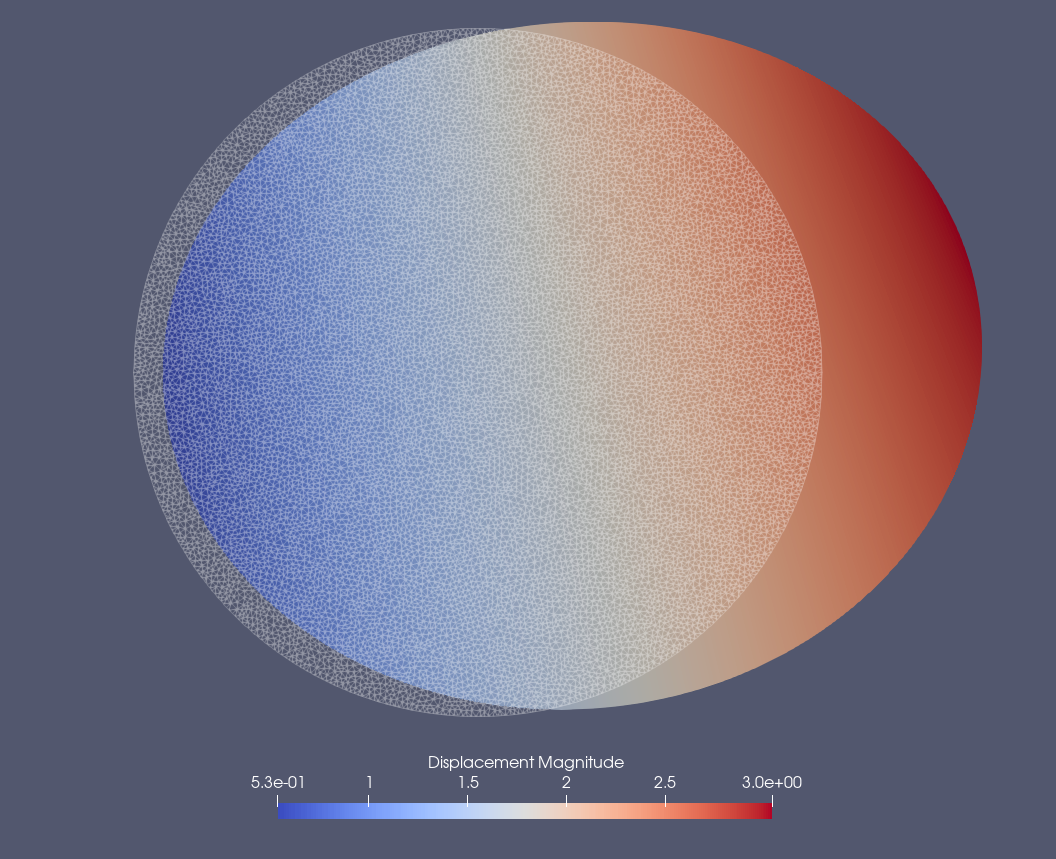
\includegraphics[width=\textwidth]{ClassicElasPara2.png}
          \caption{Classic FEM}
        \end{subfigure}
        \begin{subfigure}{0.21\textwidth}
            % \centering
            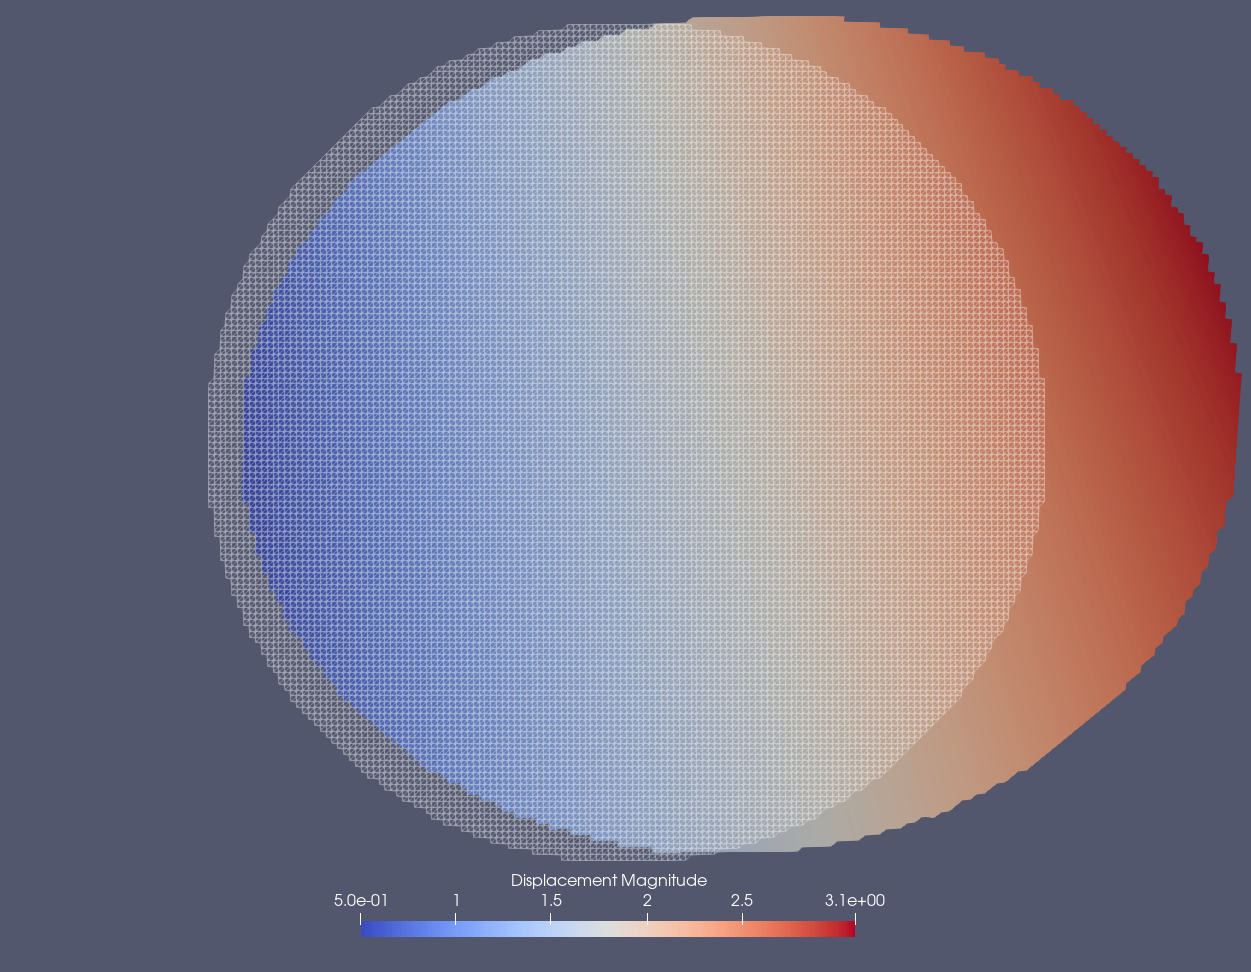
\includegraphics[width=\textwidth]{StabElasPara2.png}
          \caption{\phifem}
        \end{subfigure}
        \caption{Solution warped by vector in Paraview.}
    \end{figure}
    
    
\end{frame}

\begin{frame}
    \frametitle{Convergence study for the elasticity equation}

\begin{columns}
    \begin{column}{0.48\textwidth}
        \centering
        \begin{figure}            
        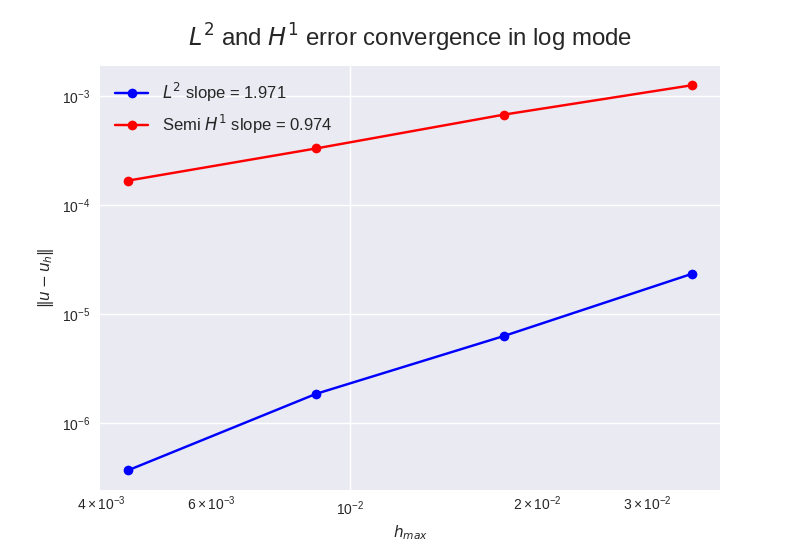
\includegraphics[width=0.95\textwidth]{ClassicElasCvg.png}
        \caption{Classic FEM}
        \end{figure}
    \end{column}
    \begin{column}{0.48\textwidth}
        \centering
        \begin{figure}            
        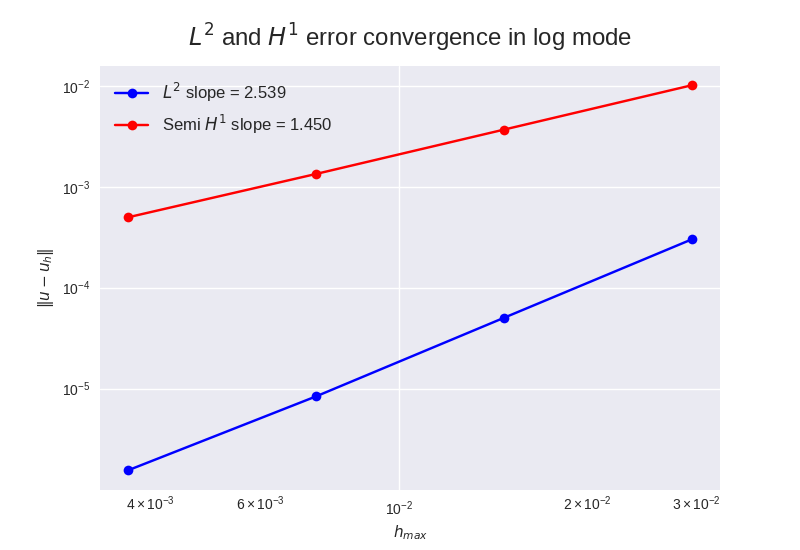
\includegraphics[width=0.95\textwidth]{StabElasCvg.png}
        \caption{\phifem}
        \end{figure}
    \end{column}
\end{columns}

\note{Rappeller qu'il s'agit des semi-normes H1.}

\begin{table}[h!]
    \centering
    \begin{tabular}{c| l| c| c}
        \toprule
        \tabhead{Problem} & \tabhead{Technique} & \tabhead{$L^2$ slope} & \tabhead{$H^1$ slope} \\
        \midrule
        \multirow{2}{4em}{Elasticity} & Classic FEM & 1.971 & 0.974 \\
         & \phifem & 2.539 & 1.450 \\
        \bottomrule
    \end{tabular}
    \caption{Convergence rates.}
\end{table}

  
\end{frame}
